\documentclass[12pt]{article} 

\usepackage{amsmath,amssymb,amsfonts}
\usepackage{psfrag}
\usepackage{color}
\definecolor{darkblue}{rgb}{0.1,0.1,.7}
\usepackage[colorlinks, linkcolor=darkblue, citecolor=darkblue, urlcolor=darkblue, linktocpage]{hyperref} 
\usepackage[square, comma, compress,numbers]{natbib}
\usepackage[]{amsmath}
\usepackage[]{graphicx}
\usepackage[]{latexsym}
\usepackage{geometry}
\usepackage{amscd}
\usepackage[all,cmtip]{xy}
\usepackage{mathrsfs}
\usepackage[margin=10pt,font=small,labelfont=bf]{caption}
\geometry{verbose,letterpaper,tmargin=2.5cm,bmargin=2.5cm,lmargin=2.6cm,rmargin=2.6cm}
\usepackage{dsdshorthand}
\usepackage{changepage}
\usepackage{listings}
\setlength{\parskip}{0.1in}
\hyphenpenalty=1000

\numberwithin{equation}{section}

\renewcommand{\be}{\begin{eqnarray}}
\renewcommand{\ee}{\end{eqnarray}}
\newcommand\nn{\nonumber}
\newcommand\cS{\mathcal{S}}
\newcommand\cR{\mathcal{R}}
\newcommand\SDPAGMP{\texttt{SDPA-GMP}}
\newcommand\SDPB{\texttt{SDPB}}
\newcommand\repl[1]{$\langle$\textrm{\em #1}$\rangle$}
\newcommand\defn[1]{\textrm{\em #1}\ $\equiv$}


\begin{document}

{\Large
\begin{center}
{\bf SDPB 2.4.0 \\\vspace{.1in}}
\end{center}
}
\begin{center}
\noindent \today
\end{center}
\tableofcontents

\section{Introduction}

\SDPB\ is an arbitrary-precision semidefinite program solver, specialized for ``polynomial matrix programs" (defined below).  This document describes \SDPB's usage and input/output.  Much more detail about its design is given in \cite{DSD}. The reader is encouraged to look there for a better understanding of \SDPB's parameters and internal operation.

\subsection{Installation and Requirements}

See \texttt{Install.md} for up-to-date instructions on getting
pre-made binaries or building from source.

\section{Polynomial Matrix Programs}
\label{sec:PMP}

\SDPB\ solves the following type of problem, which we call a {\it polynomial matrix program} (PMP).  Consider a collection of symmetric polynomial matrices
\be
M_j^n(x) &=& \begin{pmatrix}
P_{j,11}^{n}(x) & \dots & P_{j,1m_j}^{n}(x)\\
\vdots & \ddots & \vdots\\
P_{j,m_j1}^{n}(x) & \dots & P^{n}_{j,m_jm_j}(x)
\end{pmatrix}
\ee
labeled by $0 \leq n \leq N$ and $1 \leq j \leq J$,
where each element $P_{j,rs}^{n}(x)$ is a polynomial in $x$.  
Given $b\in \R^N$, we would like to
\be
\label{eq:PMPconstraint}
\begin{array}{ll}
\textrm{maximize} & b_0+b\.y\quad\textrm{over}\quad y \in \R^N,\\
\textrm{such that} & M^0_j(x)+\sum_{n=1}^{N} y_n M^n_j(x) \succeq 0 \quad \textrm{for all $x\geq 0$ and $1 \leq j \leq J$}.
\end{array}
\ee
The notation $M\succeq 0$ means ``$M$ is positive semidefinite."



\section{Input to \SDPB}

\SDPB\ takes the following input:
\begin{itemize}
\item for each $j=1,\dots,J$:
\begin{itemize}
\item polynomial matrices $M^0_j(x),\dots,M^N_j(x)$ of maximum degree $d_j$,
\item bilinear bases $q_m^{(j)}(x)$ ($m=0,\dots,\lfloor d_j/2\rfloor$),
\item sample points $x_k^{(j)}$ ($k=0,\dots,d_j$),
\item sample scalings $s_k^{(j)}$ ($k=0,\dots,d_j$),
\end{itemize}
\item an objective function $b_0\in \R$ and $b\in \R^N$.
\end{itemize}
A bilinear basis is a collection of polynomials $q_m^{(j)}(x)$ such that $\deg q_m^{(j)} = m$, for example monomials $q_m^{(j)}(x)=x^m$.  (A better choice for numerical stability is usually orthogonal polynomials on the positive real line.)  The sample points and sample scalings determine how the PMP is represented internally as an SDP.  In principle, they do not affect the solution of the PMP, but in practice they can affect numerical stability.  The constant $b_0$ is completely irrelevant to the solution algorithm, but is included for convenience.  See \cite{DSD} for details.

\subsection{Input Format}

\SDPB\ reads the data above in the following XML format.

\begin{lstlisting}[
  caption={XML input format for \SDPB},
  label=xmlinputformat,
  mathescape,
  columns=fullflexible,
  frame=single,
  escapeinside=@@,
  basicstyle=\small\ttfamily\selectfont,
]
@\defn{input to \SDPB}@
  <sdp>
    @\repl{xml for objective}@
    @\repl{xml for polynomial vector matrices}@
  </sdp>

@\defn{xml for objective}@
  <objective>
    <elt>$b_0$</elt>
    ...
    <elt>$b_N$</elt>
  </objective>
  
@\defn{xml for polynomial vector matrices}@
  <polynomialVectorMatrices>
    @\repl{xml for polynomial vector matrix $M_1^n(x)$}@
    ...
    @\repl{xml for polynomial vector matrix $M_J^n(x)$}@
  </polynomialVectorMatrices>

@\defn{xml for polynomial vector matrix $M_j^n(x)$}@
  <polynomialVectorMatrix>
    <rows>$m_j$</rows>
    <cols>$m_j$</cols>
    <elements>
      @\repl{xml for polynomial vector $P^{n}_{j,11}(x)$}@
      ...
      @\repl{xml for polynomial vector $P^{n}_{j,m_j1}(x)$}@
      ...
      @\repl{xml for polynomial vector $P^{n}_{j,1m_j}(x)$}@
      ...
      @\repl{xml for polynomial vector $P^{n}_{j,m_jm_j}(x)$}@
    </elements>
    <samplePoints>
      <elt>$x_0^{(j)}$</elt>
      ...
      <elt>$x_{d_j}^{(j)}$</elt>
    </samplePoints>
    <sampleScalings>
      <elt>$s_0^{(j)}$</elt>
      ...
      <elt>$s_{d_j}^{(j)}$</elt>
    </sampleScalings>
    <bilinearBasis>
      @\repl{xml for polynomial $q_0^{(j)}(x)$}@
      ...
      @\repl{xml for polynomial $q_{\lfloor d_j/2\rfloor}^{(j)}(x)$}@
    </bilinearBasis>
  </polynomialVectorMatrix>

@\defn{xml for polynomial vector $P^{n}_{j,rs}(x)$}@
  <polynomialVector>
    @\repl{xml for polynomial $P^{0}_{j,rs}(x)$}@
    ...
    @\repl{xml for polynomial $P^{N}_{j,rs}(x)$}@
  </polynomialVector>

@\defn{xml for polynomial $a_0+a_1 x+\dots a_d x^d$}@
  <polynomial>
    <coeff>$a_0$</coeff>
    ...
    <coeff>$a_d$</coeff>
  </polynomial>
\end{lstlisting}

The data can be spread over multiple files. In such cases the different input files should all follow the above format except that $\langle${\it xml for objective}$\rangle$ should be omitted from all but one file. The parser will combine the constraints from all the polynomial vector matrices specified in the different files.

Several aspects of the input format are inefficient.  Because the matrices are symmetric, \texttt{rows} and \texttt{cols} are redundant, and most elements are listed twice.  Also, XML is extremely verbose.

To improve performance for large inputs, the XML files must first be
preprocessed into a more efficient format.  Instructions on how to
preprocess the input and run SDPB are in \texttt{docs/Usage.md}.

\subsection{\texttt{JSON} and \texttt{Mathematica} Interface}

The program \texttt{sdp2input} generates preprocessed input files from
\texttt{JSON} or \texttt{Mathematica} data.
It automatically makes sensible choices for the bilinear bases
$q_m^{(j)}(x)$, the sample points $x_k^{(j)}$ and the sample scalings
$s_k^{(j)}$.  If you wish to experiment with these choices, there is
also an included \texttt{Mathematica} notebook \texttt{SDPB.m}.

The \texttt{Mathematica} definition of a PMP is slightly different but trivially equivalent to (\ref{eq:PMPconstraint}).  It is:
\be
\label{eq:PMPconstraintMathematica}
\begin{array}{ll}
\textrm{maximize} & a\.z\quad\textrm{over}\quad z \in \R^{N+1},\\
\textrm{such that} & \sum_{n=0}^{N} z_n W^n_j(x) \succeq 0 \quad \textrm{for all $x\geq 0$ and $1 \leq j \leq J$},\\
 & n\.z = 1.
\end{array}
\ee
where $W_j^n(x)$ are matrix polynomials.  The normalization condition $n\.z=1$ can be used to solve for one of the components of $z$ in terms of the others.  Calling the remaining components $y\in \R^N$, we arrive at (\ref{eq:PMPconstraint}), where $M_j^n(x)$ are linear combinations of $W^n_j(x)$ and $b_0,b_n$ are linear combinations of the $a_n$.  This difference in convention is for convenient use in the conformal bootstrap.

\texttt{SDPB.m} defines a function \texttt{WriteBootstrapSDP[file, sdp]}, where \texttt{file} is the XML file to be written to, and \texttt{sdp} has the following form, where the polynomials $Q^n_{j,rs}(x)$ are the elements of $W_j^n(x)$.

\begin{lstlisting}[
  caption={Usage of \texttt{WriteBootstrapSDP} in \texttt{SDPB.m}},
  mathescape,
  columns=fullflexible,
  frame=single,
  escapeinside=@@,
  basicstyle=\small\ttfamily\selectfont,
]
@\defn{function call}@ WriteBootstrapSDP[file, @\repl{sdp}@]

@\defn{sdp}@ SDP[@\repl{objective}@, @\repl{normalization}@, @\repl{positive matrices with prefactors}@]

@\defn{objective}@ {$a_0$, ..., $a_N$}

@\defn{normalization}@ {$n_0$, ..., $n_N$}

@\defn{positive matrices with prefactors}@ {
    @\repl{positive matrix with prefactor 1}@,
    ...
    @\repl{positive matrix with prefactor $J$}@,
  }

@\defn{positive matrix with prefactor $j$}@
  PositiveMatrixWithPrefactor[@\repl{prefactor}@,
    {
      {
        {$Q^0_{j,11}(x)$, ..., $Q^N_{j,11}(x)$},  ..., {$Q^0_{j,m_j1}(x)$, ..., $Q^N_{j,m_j1}(x)$}
      },
      ...
      {
        {$Q^0_{j,1m_j}(x)$, ..., $Q^N_{j,1m_j}(x)$},  ..., {$Q^0_{j,m_jm_j}(x)$, ..., $Q^N_{j,m_jm_j}(x)$}
      },
    }
  ]
  
@\defn{prefactor}@
    DampedRational[$c$, {$p_1,\dots,p_k$}, $b$, x]
  @\textrm{\em or}@
    const  
\end{lstlisting}

The prefactor in \texttt{PositiveMatrixWithPrefactor} is used for constructing bilinear bases and sample scalings.  Specifically, if the prefactor is $\chi(x)$, the bilinear basis is a set of orthogonal polynomials with respect to measure $\chi(x)dx$ on the positive real line, and sample scalings are $\chi(x_k)$, where the $x_k$ are sample points.
 The notebook \texttt{SDPB.m} only deals with damped-rational prefactors because these are relevant to the conformal bootstrap.  These stand for
\be
\texttt{DampedRational[$c$, \{$p_1,\dots,p_k$\}, $b$, $x$]} &\to& c\frac{b^x}{\prod_{i=1}^k (x-p_i)}.
\ee
We do not use an exponential-times-rational \texttt{Mathematica} function directly because the  \texttt{DampedRational} data structure makes it easier to extract information needed to construct a bilinear basis.  The notebook \texttt{SDPB.m} makes a choice of sample points that are reasonable for conformal bootstrap applications.

As an example bootstrap application, the included notebook \texttt{Bootstrap2dExample.m} computes a single-correlator dimension bound for 2d CFTs with a $\Z_2$ symmetry, as in \cite{Rychkov:2009ij}.

The \texttt{JSON} format is described by the schema in \texttt{docs/sdp2input\_schema.json}.

\subsection{An Example}
\label{sec:example}

Let's look at an example.  Consider the following problem: maximize $-y$ such that
\be
\label{eq:exampleproblem}
1+x^4 + y\p{\frac{x^4}{12} + x^2} &\geq& 0\qquad \textrm{for all $x\geq 0$}
\ee
This is an PMP with $1\x1$ positive-semidefiniteness constraints.  We will arbitrarily choose a prefactor of $e^{-x}=\texttt{DampedRational[1,\{\}, 1/E,x]}$, so that the bilinear basis consists of Laguerre polynomials.  The \texttt{Mathematica} code for this example is

\begin{lstlisting}[
  caption={Mathematica input for the example~(\ref{eq:exampleproblem})},
  label=mathematicaexample,
  mathescape,
  columns=fullflexible,
  frame=single,
  escapeinside=@@,
  basicstyle=\small\ttfamily\selectfont,
]
Module[
  {
    pols = {
      PositiveMatrixWithPrefactor[
        DampedRational[1,{}, 1/E,x],
        {{{1 + x^4, x^4/12 + x^2}}}
      ]
    },
    norm = {1, 0},
    obj  = {0, -1}
  },
  WriteBootstrapSDP["test.xml", SDP[obj, norm, pols]];
];
\end{lstlisting}
It produces the following XML file
\begin{lstlisting}[
  caption={XML file \texttt{test.xml} produced by listing~\ref{mathematicaexample}.  Decimals are truncated at 12 digits.},
  label=exampleinputfile,
  mathescape,
  columns=fullflexible,
  frame=single,
  escapeinside=@@,
  basicstyle=\footnotesize\ttfamily\selectfont,
]
<sdp>
  <objective><elt>0</elt><elt>-1</elt></objective>
  <polynomialVectorMatrices>
    <polynomialVectorMatrix>
      <rows>1</rows>
      <cols>1</cols>
      <elements>
        <polynomialVector>
          <polynomial>
            <coeff>1</coeff><coeff>0</coeff><coeff>0</coeff>
            <coeff>0</coeff><coeff>1</coeff>
          </polynomial>
          <polynomial>
            <coeff>0</coeff><coeff>0</coeff><coeff>1</coeff>
            <coeff>0</coeff><coeff>0.0833333333333</coeff>
          </polynomial>
        </polynomialVector>
      </elements>
      <samplePoints>
        <elt>0.017496844815</elt><elt>0.157471603340</elt><elt>0.857345395967</elt>
        <elt>2.117118222694</elt><elt>3.936790083523</elt>
      </samplePoints>
      <sampleScalings>
        <elt>0.982655336118</elt><elt>0.854301072560</elt><elt>0.424286902403</elt>
        <elt>0.120378031823</elt><elt>0.019510742190</elt>
      </sampleScalings>
      <bilinearBasis>
        <polynomial><coeff>1</coeff></polynomial>
        <polynomial><coeff>-1</coeff><coeff>1</coeff></polynomial>
        <polynomial><coeff>1</coeff><coeff>-2</coeff><coeff>0.5</coeff></polynomial>
      </bilinearBasis>
    </polynomialVectorMatrix>
  </polynomialVectorMatrices>
</sdp>
\end{lstlisting}

\section{Internal SDP}
\label{sec:translationPMPtoSDP}

To understand the output of \SDPB, we need a rough understanding of its internal representation of the above PMP as a semidefinite program (SDP).  Much more detail is given in \cite{DSD}.
The PMP (\ref{eq:PMPconstraint}) is translated into a dual pair of SDPs of the following form:
\be
\label{eq:traditionalSDP}
\begin{array}{rll}
\cD: & \textrm{maximize} & \Tr(CY) + b_0 + b \. y \quad \textrm{over} \quad y\in \R^N,\ Y\in \cS^K, \\
& \textrm{such that} & \Tr(A_* Y)+By = c,\ \textrm{and}\\
& Y \succeq 0.
\end{array}
\ee 
\be
\label{eq:primaldualproblems}
\begin{array}{rll}
\mathcal{P}: & \textrm{minimize} & b_0+c\.x \quad \textrm{over}\quad x\in \R^P,\ X\in \cS^K,\\
& \textrm{such that} & X= \sum_{p=1}^P A_p x_p - C,\\
& &  B^T x= b,\\
& &  X\succeq 0,
\end{array}
\ee
where ``$\succeq 0$" means ``is positive-semidefinite" and
\be
c &\in& \R^P, \nn\\
B &\in& \R^{P\x N}, \nn\\
A_1,\dots,A_P,C &\in& \cS^K.
\ee
Here, $\cS^K$ is the space of $K\x K$ symmetric real matrices, and $\Tr(A_* Y)$ denotes the vector $(\Tr(A_1 Y),\dots,\Tr(A_P Y))\in\R^P$.  An optimal solution to (\ref{eq:traditionalSDP}) and (\ref{eq:primaldualproblems}) is characterized by $XY=0$ and also equality of the primal and dual objective functions $\Tr(CY)+b_0+b\.y=b_0+c\.x$.

The residues
\be
\label{eq:residues}
P &\equiv& \sum_i A_i x_i - X - C, \nn\\
p &\equiv& b - B^T x, \nn\\
d &\equiv& c - \Tr(A_* Y) - B y,
\ee
measure the failure of $x,X,y,Y$ to satisfy their constraints.  We say a point $q=(x,X,y,Y)$ is ``primal feasible" or ``dual feasible" if the residues are sufficiently small, 
\be
\begin{array}{rrcccl}
\textrm{primal feasible:} & \texttt{primalError} &\equiv& \max_{i,j}\{|p_i|, |P_{ij}|\} &<& \texttt{primalErrorThreshold};\\
\textrm{dual feasible:} & \texttt{dualError} &\equiv&\max_i\{|d_i|\} &<& \texttt{dualErrorThreshold},\nn\\
\end{array}
\ee
where $\texttt{primalErrorThreshold}\ll 1$ and $\texttt{dualErrorThreshold} \ll 1$ are parameters chosen by the user.

An optimal point should be both primal and dual feasible, and have (nearly) equal primal and dual objective values.  Specifically, let us define $\texttt{dualityGap}$ as the normalized difference between the primal and dual objective functions
\be
\texttt{dualityGap} &\equiv& \frac{|\texttt{primalObjective} - \texttt{dualObjective}|}{\max\{1, |\texttt{primalObjective} + \texttt{dualObjective}|\}}, \nn\\
\texttt{primalObjective} &\equiv& b_0+c\. x, \nn\\
\texttt{dualObjective} &\equiv& \Tr(CY)+b_0+b\.y.
\ee
A point is considered ``optimal" if
\be
\texttt{dualityGap} &<& \texttt{dualityGapThreshold},
\ee
where $\texttt{dualityGapThreshold} \ll 1$ is chosen by the user.


\section{Output of \SDPB}

\subsection{Terminal Output}

The output from running \SDPB\ on the example problem in section~\ref{sec:example} is in listing~\ref{listing:exampleoutput}.  The input, output, and checkpoint files are listed first, followed by various parameters.  After each iteration, \SDPB\ prints the following:
\begin{description}
\item[\texttt{time}:] The current solver runtime in seconds.
\item[\texttt{mu}:] The value of the complementarity $\Tr(XY)/K$.
\item[\texttt{P-obj}:] The primal objective value $b_0+c\.x$.
\item[\texttt{D-obj}:] The dual objective value $\Tr(CY)+b_0+b\.y$.
\item[\texttt{gap}:] The value of \texttt{dualityGap}.
\item[\texttt{P-err}:] The primal error $\max_{i,j}\{|P_{ij}|\}$.
\item[\texttt{p-err}:] The primal error $\max_{i}\{|p_i||\}$.
\item[\texttt{D-err}:] The dual error $\max_i\{|d_i|\}$.
\item[\texttt{P-step}:] The primal step length $\alpha_\cP$ described in \cite{DSD}.
\item[\texttt{D-step}:] The dual step length $\alpha_\cD$ described in \cite{DSD}.
\item[\texttt{beta}:]  The corrector centering parameter $\beta_c$ described in \cite{DSD}.
\end{description}

If an optimal solution exists, the primal and dual error will decrease until the problem becomes primal and dual feasible.  Then the primal and dual objective functions start to converge, and the complementarity $\mu$ decreases until the duality gap becomes smaller than \texttt{dualityGapThreshold}.

The terminal output ends with the final values of the primal/dual objectives, primal/dual errors and duality gap.

\begin{lstlisting}[
  caption={Output of \SDPB\ for the input file in listing~\ref{exampleinputfile}},
  columns=fullflexible,
  label=listing:exampleoutput,
  keepspaces=true,
  basicstyle=\scriptsize\ttfamily\selectfont,
]
$ ./build/sdpb -s test/test --noFinalCheckpoint --procsPerNode=1
SDPB started at 2020-Jan-16 12:09:59
SDP directory   : "test/test"
out directory   : "test/test_out"
checkpoint in   : "test/test.ck"
checkpoint out  : "test/test.ck"

Parameters:
maxIterations                = 500
maxRuntime                   = 9223372036854775807
checkpointInterval           = 3600
noFinalCheckpoint            = true
writeSolution                = x,y
findPrimalFeasible           = false
findDualFeasible             = false
detectPrimalFeasibleJump     = false
detectDualFeasibleJump       = false
precision(actual)            = 400(448)
dualityGapThreshold          = 1e-30
primalErrorThreshold         = 1e-30
dualErrorThreshold           = 1e-30
initialMatrixScalePrimal     = 1e+20
initialMatrixScaleDual       = 1e+20
feasibleCenteringParameter   = 0.1
infeasibleCenteringParameter = 0.3
stepLengthReduction          = 0.7
maxComplementarity           = 1e+100
procsPerNode                 = 1
procGranularity              = 1
verbosity                    = 1

Block Grid Mapping
Node	Num Procs	Cost		Block List
==================================================
0	1		25	{(0,5)}



          time    mu     P-obj       D-obj      gap         P-err       p-err       D-err      P-step   D-step   beta
---------------------------------------------------------------------------------------------------------------------
1            0 1.0e+40  +0.00       +0.00       0.00       +1.00e+20   +1.00       +2.88e+20   0.631    0.647    0.300
2            0 5.0e+39  +9.49e+19   -1.64e+20   1.00       +3.69e+19   +0.369      +1.02e+20   0.653    0.639    0.300
3            0 2.5e+39  +1.04e+20   -2.92e+20   1.00       +1.28e+19   +0.128      +3.68e+19   0.660    0.639    0.300
4            0 1.2e+39  +1.43e+20   -4.30e+20   1.00       +4.35e+18   +0.0435     +1.33e+19   0.652    0.638    0.300
5            0 5.8e+38  +1.91e+20   -6.13e+20   1.00       +1.51e+18   +0.0151     +4.80e+18   0.645    0.636    0.300
6            0 2.8e+38  +2.52e+20   -8.65e+20   1.00       +5.38e+17   +0.00538    +1.75e+18   0.640    0.634    0.300
7            0 1.4e+38  +3.36e+20   -1.21e+21   1.00       +1.94e+17   +0.00194    +6.38e+17   0.636    0.633    0.300
8            0 7.2e+37  +4.52e+20   -1.69e+21   1.00       +7.05e+16   +0.000705   +2.34e+17   0.635    0.633    0.300
9            0 3.6e+37  +6.16e+20   -2.34e+21   1.00       +2.57e+16   +0.000257   +8.58e+16   0.634    0.633    0.300
10           0 1.8e+37  +8.43e+20   -3.23e+21   1.00       +9.43e+15   +9.43e-05   +3.15e+16   0.633    0.633    0.300
11           0 9.3e+36  +1.16e+21   -4.46e+21   1.00       +3.46e+15   +3.46e-05   +1.16e+16   0.633    0.633    0.300
12           0 4.7e+36  +1.59e+21   -6.16e+21   1.00       +1.27e+15   +1.27e-05   +4.24e+15   0.633    0.633    0.300
13           0 2.4e+36  +2.20e+21   -8.49e+21   1.00       +4.65e+14   +4.65e-06   +1.56e+15   0.633    0.633    0.300
14           0 1.2e+36  +3.03e+21   -1.17e+22   1.00       +1.71e+14   +1.71e-06   +5.71e+14   0.633    0.633    0.300
15           0 6.1e+35  +4.18e+21   -1.62e+22   1.00       +6.26e+13   +6.26e-07   +2.09e+14   0.633    0.633    0.300
16           0 3.1e+35  +5.77e+21   -2.23e+22   1.00       +2.30e+13   +2.30e-07   +7.68e+13   0.633    0.633    0.300
17           0 1.6e+35  +7.96e+21   -3.08e+22   1.00       +8.42e+12   +8.42e-08   +2.82e+13   0.633    0.633    0.300
18           0 7.9e+34  +1.10e+22   -4.25e+22   1.00       +3.09e+12   +3.09e-08   +1.03e+13   0.633    0.633    0.300
19           0 4.0e+34  +1.52e+22   -5.86e+22   1.00       +1.13e+12   +1.13e-08   +3.79e+12   0.633    0.633    0.300
20           0 2.0e+34  +2.09e+22   -8.09e+22   1.00       +4.15e+11   +4.15e-09   +1.39e+12   0.633    0.633    0.300
21           0 1.0e+34  +2.89e+22   -1.12e+23   1.00       +1.52e+11   +1.52e-09   +5.09e+11   0.633    0.633    0.300
22           0 5.2e+33  +3.98e+22   -1.54e+23   1.00       +5.58e+10   +5.58e-10   +1.87e+11   0.633    0.633    0.300
23           0 2.6e+33  +5.50e+22   -2.13e+23   1.00       +2.05e+10   +2.05e-10   +6.85e+10   0.633    0.633    0.300
24           0 1.3e+33  +7.59e+22   -2.93e+23   1.00       +7.51e+09   +7.51e-11   +2.51e+10   0.633    0.633    0.300
25           0 6.7e+32  +1.05e+23   -4.05e+23   1.00       +2.75e+09   +2.75e-11   +9.21e+09   0.633    0.633    0.300
26           0 3.4e+32  +1.44e+23   -5.59e+23   1.00       +1.01e+09   +1.01e-11   +3.38e+09   0.633    0.633    0.300
27           0 1.7e+32  +1.99e+23   -7.71e+23   1.00       +3.70e+08   +3.70e-12   +1.24e+09   0.633    0.633    0.300
28           0 8.7e+31  +2.75e+23   -1.06e+24   1.00       +1.36e+08   +1.36e-12   +4.54e+08   0.633    0.633    0.300
29           0 4.4e+31  +3.80e+23   -1.47e+24   1.00       +4.98e+07   +4.98e-13   +1.67e+08   0.633    0.633    0.300
30           0 2.2e+31  +5.24e+23   -2.03e+24   1.00       +1.83e+07   +1.83e-13   +6.11e+07   0.633    0.633    0.300
31           0 1.1e+31  +7.23e+23   -2.80e+24   1.00       +6.70e+06   +6.70e-14   +2.24e+07   0.633    0.633    0.300
32           0 5.7e+30  +9.98e+23   -3.86e+24   1.00       +2.46e+06   +2.46e-14   +8.22e+06   0.633    0.633    0.300
33           0 2.9e+30  +1.38e+24   -5.32e+24   1.00       +9.01e+05   +9.01e-15   +3.01e+06   0.633    0.633    0.300
34           0 1.5e+30  +1.90e+24   -7.35e+24   1.00       +3.30e+05   +3.30e-15   +1.11e+06   0.633    0.633    0.300
35           0 7.4e+29  +2.62e+24   -1.01e+25   1.00       +1.21e+05   +1.21e-15   +4.05e+05   0.633    0.633    0.300
36           0 3.7e+29  +3.62e+24   -1.40e+25   1.00       +4.44e+04   +4.44e-16   +1.49e+05   0.633    0.633    0.300
37           0 1.9e+29  +4.99e+24   -1.93e+25   1.00       +1.63e+04   +1.63e-16   +5.45e+04   0.633    0.633    0.300
38           0 9.6e+28  +6.89e+24   -2.66e+25   1.00       +5.98e+03   +5.98e-17   +2.00e+04   0.633    0.633    0.300
39           0 4.8e+28  +9.51e+24   -3.68e+25   1.00       +2.19e+03   +2.19e-17   +7.33e+03   0.633    0.633    0.300
40           0 2.4e+28  +1.31e+25   -5.07e+25   1.00       +803.       +8.03e-18   +2.69e+03   0.634    0.634    0.300
41           0 1.2e+28  +1.81e+25   -7.00e+25   1.00       +294.       +2.94e-18   +985.       0.634    0.634    0.300
42           0 6.3e+27  +2.50e+25   -9.64e+25   1.00       +108.       +1.08e-18   +360.       0.636    0.635    0.300
43           0 3.2e+27  +3.44e+25   -1.32e+26   1.00       +39.1       +3.91e-19   +131.       0.642    0.639    0.300
44           0 1.6e+27  +4.72e+25   -1.81e+26   1.00       +14.0       +1.40e-19   +47.5       0.657    0.649    0.300
45           0 7.8e+26  +6.42e+25   -2.41e+26   1.00       +4.80       +4.80e-20   +16.7       0.699    0.677    0.300
46           0 3.6e+26  +8.51e+25   -3.04e+26   1.00       +1.44       +1.44e-20   +5.40       0.785    0.768    0.300
47           0 1.6e+26  +1.02e+26   -3.19e+26   1.00       +0.310      +3.10e-21   +1.25       1.00     1.00     0.300
48           0 5.3e+25  +8.01e+25   -1.83e+26   1.00       +1.16e-115  +4.30e-120  +7.84e-90   0.734    0.734    0.100
49           0 1.8e+25  +2.73e+25   -6.20e+25   1.00       +7.61e-116  +2.83e-117  +1.35e-85   0.736    0.736    0.100
50           0 6.0e+24  +9.21e+24   -2.09e+25   1.00       +1.27e-115  +1.74e-116  +5.21e-86   0.736    0.736    0.100
51           0 2.0e+24  +3.10e+24   -7.08e+24   1.00       +1.30e-115  +2.40e-116  +1.44e-86   0.736    0.736    0.100
52           0 6.9e+23  +1.04e+24   -2.39e+24   1.00       +1.27e-115  +1.24e-116  +4.03e-87   0.737    0.737    0.100
53           0 2.3e+23  +3.51e+23   -8.08e+23   1.00       +1.18e-115  +5.06e-118  +1.08e-87   0.737    0.737    0.100
54           0 7.8e+22  +1.18e+23   -2.72e+23   1.00       +1.05e-115  +8.09e-118  +2.86e-88   0.738    0.738    0.100
55           0 2.6e+22  +3.95e+22   -9.14e+22   1.00       +1.02e-115  +3.81e-117  +7.51e-89   0.738    0.738    0.100
56           0 8.8e+21  +1.32e+22   -3.07e+22   1.00       +1.49e-115  +1.50e-117  +1.97e-89   0.739    0.739    0.100
57           0 2.9e+21  +4.43e+21   -1.03e+22   1.00       +1.27e-115  +1.14e-116  +5.14e-90   0.739    0.739    0.100
58           0 9.8e+20  +1.48e+21   -3.44e+21   1.00       +1.02e-115  +1.35e-116  +1.34e-90   0.739    0.739    0.100
59           0 3.3e+20  +4.95e+20   -1.15e+21   1.00       +1.02e-115  +1.40e-117  +3.50e-91   0.740    0.740    0.100
60           0 1.1e+20  +1.66e+20   -3.85e+20   1.00       +9.59e-116  +6.80e-118  +9.11e-92   0.740    0.740    0.100
61           0 3.7e+19  +5.54e+19   -1.29e+20   1.00       +1.02e-115  +2.37e-118  +2.37e-92   0.740    0.740    0.100
62           0 1.2e+19  +1.85e+19   -4.30e+19   1.00       +8.41e-116  +6.29e-119  +6.17e-93   0.740    0.740    0.100
63           0 4.1e+18  +6.18e+18   -1.44e+19   1.00       +5.21e-116  +6.30e-120  +1.61e-93   0.740    0.740    0.100
64           0 1.4e+18  +2.06e+18   -4.80e+18   1.00       +1.36e-116  +1.64e-120  +4.17e-94   0.740    0.740    0.100
65           0 4.6e+17  +6.89e+17   -1.60e+18   1.00       +3.52e-117  +4.26e-121  +1.09e-94   0.740    0.740    0.100
66           0 1.5e+17  +2.30e+17   -5.36e+17   1.00       +9.16e-118  +1.11e-121  +2.82e-95   0.740    0.740    0.100
67           0 5.1e+16  +7.68e+16   -1.79e+17   1.00       +2.38e-118  +2.88e-122  +7.33e-96   0.740    0.740    0.100
68           0 1.7e+16  +2.56e+16   -5.97e+16   1.00       +6.18e-119  +7.54e-123  +1.90e-96   0.740    0.740    0.100
69           0 5.7e+15  +8.56e+15   -1.99e+16   1.00       +1.61e-119  +2.03e-123  +4.95e-97   0.740    0.740    0.100
70           0 1.9e+15  +2.86e+15   -6.65e+15   1.00       +4.17e-120  +7.30e-124  +1.29e-97   0.740    0.740    0.100
71           0 6.3e+14  +9.53e+14   -2.22e+15   1.00       +1.08e-120  +4.46e-124  +3.34e-98   0.740    0.740    0.100
72           0 2.1e+14  +3.18e+14   -7.41e+14   1.00       +2.82e-121  +4.55e-124  +8.67e-99   0.740    0.740    0.100
73           0 7.1e+13  +1.06e+14   -2.47e+14   1.00       +7.31e-122  +1.18e-124  +2.25e-99   0.740    0.740    0.100
74           0 2.4e+13  +3.54e+13   -8.26e+13   1.00       +1.90e-122  +3.07e-125  +5.85e-100  0.740    0.740    0.100
75           0 7.9e+12  +1.18e+13   -2.76e+13   1.00       +4.93e-123  +7.98e-126  +1.52e-100  0.740    0.740    0.100
76           0 2.6e+12  +3.94e+12   -9.20e+12   1.00       +1.28e-123  +2.07e-126  +3.94e-101  0.740    0.740    0.100
77           0 8.8e+11  +1.32e+12   -3.07e+12   1.00       +3.33e-124  +5.38e-127  +1.02e-101  0.740    0.740    0.100
78           0 2.9e+11  +4.39e+11   -1.02e+12   1.00       +8.63e-125  +1.40e-127  +2.66e-102  0.740    0.740    0.100
79           0 9.8e+10  +1.47e+11   -3.42e+11   1.00       +2.24e-125  +3.63e-128  +6.90e-103  0.740    0.740    0.100
80           0 3.3e+10  +4.89e+10   -1.14e+11   1.00       +5.82e-126  +9.42e-129  +1.79e-103  0.740    0.740    0.100
81           0 1.1e+10  +1.63e+10   -3.80e+10   1.00       +1.51e-126  +2.44e-129  +4.65e-104  0.740    0.740    0.100
82           0 3.6e+09  +5.44e+09   -1.27e+10   1.00       +3.92e-127  +6.35e-130  +1.21e-104  0.740    0.740    0.100
83           0 1.2e+09  +1.82e+09   -4.24e+09   1.00       +1.02e-127  +1.65e-130  +3.14e-105  0.740    0.740    0.100
84           0 4.0e+08  +6.06e+08   -1.41e+09   1.00       +2.65e-128  +4.28e-131  +8.15e-106  0.740    0.740    0.100
85           0 1.3e+08  +2.02e+08   -4.72e+08   1.00       +6.87e-129  +1.11e-131  +2.11e-106  0.740    0.740    0.100
86           0 4.5e+07  +6.75e+07   -1.57e+08   1.00       +1.78e-129  +2.88e-132  +5.49e-107  0.740    0.740    0.100
87           0 1.5e+07  +2.25e+07   -5.25e+07   1.00       +4.63e-130  +7.48e-133  +1.43e-107  0.740    0.740    0.100
88           0 5.0e+06  +7.51e+06   -1.75e+07   1.00       +1.20e-130  +1.95e-133  +3.70e-108  0.740    0.740    0.100
89           0 1.7e+06  +2.51e+06   -5.85e+06   1.00       +3.12e-131  +5.16e-134  +9.61e-109  0.740    0.740    0.100
90           0 5.6e+05  +8.36e+05   -1.95e+06   1.00       +8.10e-132  +1.17e-134  +2.49e-109  0.740    0.740    0.100
91           0 1.9e+05  +2.79e+05   -6.51e+05   1.00       +2.10e-132  +4.64e-135  +6.48e-110  0.740    0.740    0.100
92           0 6.2e+04  +9.31e+04   -2.17e+05   1.00       +5.37e-133  +3.64e-136  +1.68e-110  0.740    0.740    0.100
93           0 2.1e+04  +3.11e+04   -7.24e+04   1.00       +1.39e-133  +3.38e-136  +4.36e-111  0.740    0.740    0.100
94           0 6.9e+03  +1.04e+04   -2.41e+04   1.00       +3.58e-134  +0.00       +1.13e-111  0.741    0.741    0.100
95           0 2.3e+03  +3.47e+03   -8.04e+03   1.00       +6.87e-135  +0.00       +2.94e-112  0.741    0.741    0.100
96           0 7.7e+02  +1.17e+03   -2.67e+03   1.00       +4.30e-135  +0.00       +7.63e-113  0.741    0.741    0.100
97           0 2.6e+02  +394.       -886.       1.00       +5.50e-135  +2.91e-135  +1.98e-113  0.741    0.741    0.100
98           0 85.      +136.       -291.       1.00       +8.25e-135  +1.38e-135  +5.13e-114  0.738    0.738    0.100
99           0 29.      +49.8       -93.6       1.00       +6.88e-135  +0.00       +1.34e-114  0.722    0.722    0.100
100          0 10.      +21.0       -29.2       1.00       +7.73e-135  +2.19e-136  +3.74e-115  0.694    0.694    0.100
101          0 3.8      +10.5       -8.33       1.00       +7.87e-135  +3.67e-136  +1.14e-115  0.707    0.707    0.100
102          0 1.4      +5.45       -1.41       1.00       +6.88e-135  +1.10e-135  +3.35e-116  0.765    0.765    0.100
103          0 0.43     +2.99       +0.854      0.555      +6.88e-135  +1.42e-135  +7.86e-117  0.768    0.768    0.100
104          0 0.13     +2.20       +1.54       0.176      +4.49e-135  +2.22e-136  +1.83e-117  0.764    0.764    0.100
105          0 0.041    +1.95       +1.75       0.0557     +3.12e-136  +0.00       +4.32e-118  0.764    0.764    0.100
106          0 0.013    +1.88       +1.81       0.0175     +7.73e-136  +0.00       +1.02e-118  0.766    0.766    0.100
107          0 0.0040   +1.85       +1.83       0.00543    +7.83e-136  +0.00       +2.38e-119  0.768    0.768    0.100
108          0 0.0012   +1.84       +1.84       0.00168    +7.53e-137  +0.00       +5.52e-120  0.770    0.770    0.100
109          0 0.00038  +1.84       +1.84       0.000514   +2.78e-136  +0.00       +1.27e-120  0.772    0.772    0.100
110          0 0.00012  +1.84       +1.84       0.000157   +2.01e-136  +0.00       +2.89e-121  0.773    0.773    0.100
111          0 3.5e-05  +1.84       +1.84       4.77e-05   +1.06e-135  +0.00       +6.55e-122  0.774    0.774    0.100
112          0 1.1e-05  +1.84       +1.84       1.44e-05   +1.91e-136  +0.00       +1.48e-122  0.775    0.775    0.100
113          0 3.2e-06  +1.84       +1.84       4.37e-06   +1.03e-135  +2.48e-137  +3.32e-123  0.776    0.776    0.100
114          0 9.7e-07  +1.84       +1.84       1.32e-06   +3.47e-136  +1.15e-137  +7.44e-124  0.776    0.776    0.100
115          0 2.9e-07  +1.84       +1.84       3.97e-07   +3.13e-136  +4.87e-137  +1.66e-124  0.777    0.777    0.100
116          0 8.8e-08  +1.84       +1.84       1.19e-07   +5.57e-136  +3.17e-136  +3.71e-125  0.777    0.777    0.100
117          0 2.6e-08  +1.84       +1.84       3.59e-08   +3.03e-136  +1.94e-136  +8.28e-126  0.777    0.777    0.100
118          0 7.9e-09  +1.84       +1.84       1.08e-08   +8.13e-137  +1.80e-136  +1.84e-126  0.777    0.777    0.100
119          0 2.4e-09  +1.84       +1.84       3.24e-09   +5.99e-136  +9.64e-137  +4.11e-127  0.777    0.777    0.100
120          0 7.2e-10  +1.84       +1.84       9.73e-10   +2.26e-136  +2.06e-136  +9.14e-128  0.778    0.778    0.100
121          0 2.2e-10  +1.84       +1.84       2.92e-10   +8.56e-136  +3.81e-136  +2.03e-128  0.778    0.778    0.100
122          0 6.5e-11  +1.84       +1.84       8.77e-11   +7.51e-136  +4.42e-136  +4.52e-129  0.778    0.778    0.100
123          0 1.9e-11  +1.84       +1.84       2.63e-11   +8.85e-136  +4.13e-136  +1.01e-129  0.778    0.778    0.100
124          0 5.8e-12  +1.84       +1.84       7.90e-12   +4.98e-136  +3.71e-136  +2.24e-130  0.778    0.778    0.100
125          0 1.7e-12  +1.84       +1.84       2.37e-12   +4.77e-136  +4.39e-136  +4.97e-131  0.778    0.778    0.100
126          0 5.2e-13  +1.84       +1.84       7.11e-13   +7.87e-136  +3.71e-136  +1.10e-131  0.778    0.778    0.100
127          0 1.6e-13  +1.84       +1.84       2.13e-13   +1.47e-136  +1.12e-136  +2.46e-132  0.778    0.778    0.100
128          0 4.7e-14  +1.84       +1.84       6.40e-14   +5.50e-136  +2.25e-136  +5.50e-133  0.778    0.778    0.100
129          0 1.4e-14  +1.84       +1.84       1.92e-14   +2.38e-136  +1.21e-136  +1.21e-133  0.778    0.778    0.100
130          0 4.2e-15  +1.84       +1.84       5.76e-15   +5.66e-136  +1.77e-136  +3.16e-134  0.778    0.778    0.100
131          0 1.3e-15  +1.84       +1.84       1.73e-15   +1.88e-136  +2.70e-136  +1.93e-134  0.778    0.778    0.100
132          0 3.8e-16  +1.84       +1.84       5.19e-16   +1.06e-135  +4.49e-136  +1.93e-134  0.778    0.778    0.100
133          0 1.1e-16  +1.84       +1.84       1.56e-16   +2.13e-136  +4.49e-136  +7.29e-134  0.778    0.778    0.100
134          0 3.4e-17  +1.84       +1.84       4.67e-17   +8.79e-136  +5.18e-136  +7.98e-134  0.778    0.778    0.100
135          0 1.0e-17  +1.84       +1.84       1.40e-17   +5.56e-136  +1.20e-136  +7.57e-134  0.778    0.778    0.100
136          0 3.1e-18  +1.84       +1.84       4.20e-18   +3.21e-136  +1.30e-136  +6.05e-134  0.778    0.778    0.100
137          0 9.3e-19  +1.84       +1.84       1.26e-18   +1.30e-136  +2.94e-136  +1.27e-133  0.778    0.778    0.100
138          0 2.8e-19  +1.84       +1.84       3.78e-19   +6.93e-136  +4.69e-136  +2.74e-133  0.778    0.778    0.100
139          0 8.4e-20  +1.84       +1.84       1.13e-19   +1.59e-136  +3.72e-136  +2.09e-133  0.778    0.778    0.100
140          0 2.5e-20  +1.84       +1.84       3.40e-20   +3.17e-136  +1.14e-136  +1.91e-133  0.778    0.778    0.100
141          0 7.5e-21  +1.84       +1.84       1.02e-20   +9.84e-136  +0.00       +1.06e-132  0.778    0.778    0.100
142          0 2.3e-21  +1.84       +1.84       3.06e-21   +4.28e-136  +0.00       +1.15e-132  0.778    0.778    0.100
143          0 6.8e-22  +1.84       +1.84       9.19e-22   +1.20e-136  +0.00       +4.95e-133  0.778    0.778    0.100
144          0 2.0e-22  +1.84       +1.84       2.76e-22   +3.46e-136  +3.39e-137  +1.33e-132  0.778    0.778    0.100
145          0 6.1e-23  +1.84       +1.84       8.27e-23   +8.21e-136  +1.37e-136  +1.18e-132  0.778    0.778    0.100
146          0 1.8e-23  +1.84       +1.84       2.48e-23   +4.89e-136  +1.26e-136  +1.52e-132  0.778    0.778    0.100
147          0 5.5e-24  +1.84       +1.84       7.44e-24   +4.39e-136  +9.00e-137  +1.11e-132  0.778    0.778    0.100
148          0 1.6e-24  +1.84       +1.84       2.23e-24   +6.16e-136  +8.19e-137  +5.68e-133  0.778    0.778    0.100
149          0 4.9e-25  +1.84       +1.84       6.70e-25   +9.19e-136  +4.69e-136  +3.13e-132  0.778    0.778    0.100
150          0 1.5e-25  +1.84       +1.84       2.01e-25   +6.83e-136  +4.32e-136  +1.99e-132  0.778    0.778    0.100
151          0 4.4e-26  +1.84       +1.84       6.03e-26   +2.69e-136  +1.71e-136  +2.12e-132  0.778    0.778    0.100
152          0 1.3e-26  +1.84       +1.84       1.81e-26   +8.64e-136  +2.15e-136  +4.23e-132  0.778    0.778    0.100
153          0 4.0e-27  +1.84       +1.84       5.43e-27   +2.11e-136  +2.48e-136  +8.79e-132  0.778    0.778    0.100
154          0 1.2e-27  +1.84       +1.84       1.63e-27   +5.05e-136  +2.04e-136  +5.63e-132  0.778    0.778    0.100
155          0 3.6e-28  +1.84       +1.84       4.88e-28   +6.08e-136  +3.21e-136  +7.22e-132  0.778    0.778    0.100
156          0 1.1e-28  +1.84       +1.84       1.47e-28   +3.22e-136  +3.50e-136  +1.84e-131  0.778    0.778    0.100
157          0 3.2e-29  +1.84       +1.84       4.40e-29   +2.57e-136  +1.04e-136  +1.74e-131  0.778    0.778    0.100
158          0 9.7e-30  +1.84       +1.84       1.32e-29   +7.44e-136  +2.75e-136  +1.38e-131  0.778    0.778    0.100
159          0 2.9e-30  +1.84       +1.84       3.96e-30   +2.35e-136  +8.75e-137  +3.78e-131  0.778    0.778    0.100
160          0 8.7e-31  +1.84       +1.84       1.19e-30   +1.01e-135  +4.53e-136  +1.55e-131  0.778    0.778    0.100
-----found primal-dual optimal solution-----

primalObjective = 1.84026576313204924668804017173055420056358532030282556465761906133430166726537336826049865612094019
0211160188629478172050928280455570379
dualObjective   = 1.84026576313204924668804017172924388084784907020307957926406455972756967820389551729116356865203683
7213248476950467408183341489981597367
dualityGap      = 3.56013718775636270149999059635335050723442743109168831293885607041894974620853522385695653183532885
8564162988744217253002402735522747108e-31
primalError     = 5.80997135339813093497058173684136107954665719646557426347572132314645807188713585157511697443878587
3209402480858514950312788893168634202e-136
dualError       = 1.46841378193538126331627470296813105467197677842025686726937628183154614032611825901779694044217367
8064808163099397434054356812427728775e-131

Saving solution to      : "test/test_out"
\end{lstlisting}

\subsection{Termination}

The possible termination reasons for \SDPB\ are as follows
\begin{description}
\item[\texttt{found primal-dual optimal solution}] \hfill\\
Found a solution for $x,X,y,Y$ that is simultaneously primal feasible, dual feasible, and optimal.
\item[\texttt{found primal feasible solution}] \hfill\\
Found a solution for $x,X$ that is primal feasible.  \SDPB\ will only terminate with this result if the option \texttt{--findPrimalFeasible} is specified.
\item[\texttt{found dual feasible solution}] \hfill\\
Found a solution for $y,Y$ that is dual feasible.  \SDPB\ will only terminate with this result if the option \texttt{--findDualFeasible} is specified.
\item[\texttt{primal feasible jump detected}] \hfill\\
A Newton step with primal step length $\alpha_\cP$ just occurred, without resulting in a primal feasible solution.  (Usually this means one should increase \texttt{precision}.)
\item[\texttt{dual feasible jump detected}] \hfill\\
A Newton step with dual step length $\alpha_\cD$ just occurred, without resulting in a dual feasible solution.  (Usually this means one should increase \texttt{precision}.)
\item[\texttt{maxIterations exceeded}] \hfill\\
\SDPB\ has run for more iterations than specified by the option \texttt{--maxIterations}.
\item[\texttt{maxRuntime exceeded}] \hfill\\
\SDPB\ has run for longer than specified by the option \texttt{--maxRuntime}.
\item[\texttt{maxComplementarity exceeded}] \hfill\\
$\mu=\Tr(XY)/\dim(X)$ exceeded the value specified by \texttt{--maxComplementarity}.  This might indicate that the problem is unbounded and no optimal solution will be found.
\end{description}

When using \SDPB\ to determine primal or dual feasibility, one can specify the options \texttt{--findPrimalFeasible} or \texttt{--findDualFeasible}.  This will cause the solver to terminate immediately once the primal or dual errors are sufficiently small.  This often occurs immediately after the primal or dual step lengths become equal to $1$.  A step length of $1$ means that the solver has found a Newton step that exactly solves the primal or dual constraints, while preserving positive-semidefiniteness of $X,Y$.  Sometimes a step length of $1$ does not result in sufficiently small primal/dual errors.  This is indicative of numerical instabilities and usually means \texttt{precision} should be increased.  The options \texttt{--detectPrimalFeasibleJump} and \texttt{--detectPrimalFeasibleJump} cause \SDPB\ to terminate if a step length of 1 occurs without resulting in primal/dual feasibility.  If desired, one can then restart the solver with a higher value of \texttt{precision}.


\subsection{Output File}

\begin{lstlisting}[
  caption={Contents of the output file \texttt{test\_out/out.txt} corresponding to listing~\ref{exampleinputfile}. Decimal expansions have been truncated for brevity.  \texttt{Mathematica} uses \texttt{*\^} instead of the character \texttt{e} for scientific notation.  Thus, the output format is not quite suitable for import into \texttt{Mathematica} without modification.  This could be changed in future versions.},
  columns=fullflexible,
  label=listing:exampleoutputfile,
  keepspaces=true,
  frame=single,
  basicstyle=\footnotesize\ttfamily\selectfont,
]
terminateReason = "found primal-dual optimal solution";
primalObjective = 1.8402657631320492466880401717305542005635853203028255646...;
dualObjective   = 1.8402657631320492466880401717292438808478490702030795792...;
dualityGap      = 3.5601371877563627014999905963533505072344274310916883129...e-31;
primalError     = 5.8099713533981309349705817368413610795466571964655742634...e-136;
dualError       = 1.4684137819353812633162747029681310546719767784202568672...e-131;
Solver runtime  = 0;
\end{lstlisting}


The output file \texttt{test\_out/out.txt} corresponding to
listing~\ref{exampleinputfile} is shown in
listing~\ref{listing:exampleoutputfile}. It includes the reason for
termination, the final primal/dual objective values, the final duality
gap, the final primal/dual errors, and the total runtime. The vector
$y$ is saved in \texttt{test\_out/y.txt}, and the two blocks of the $x$ vector
are saved in \texttt{test\_out/x\_0.txt} and
\texttt{test\_out/x\_1.txt}.  To write additional files for the matrices $X$ and $Y,$ add the
option \newline
\texttt{--writeSolution="x,y,X,Y"}.

The value of $y$ gives the solution to our optimization problem.  The function
\be
1+x^4 + (-1.840265763084)\p{\frac{x^4}{12} + x^2}
\ee
is plotted in figure~\ref{fig:plot}.  The zero near $x=1$ shows that $y$ is optimal.

\begin{figure}
\begin{center}
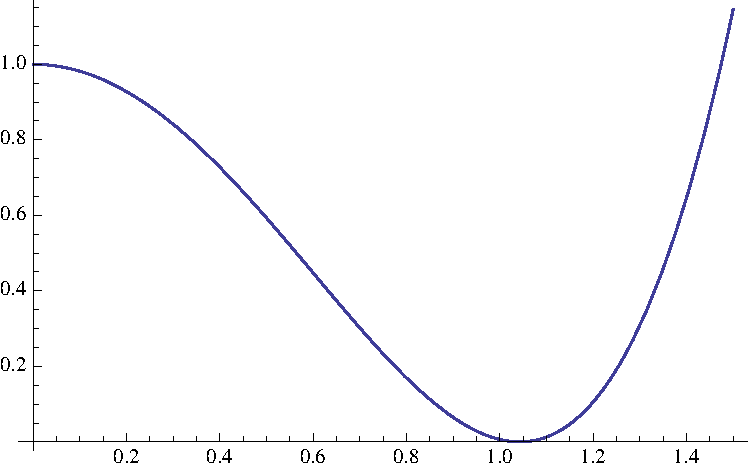
\includegraphics[width=0.7\textwidth]{optimizationplot}
\end{center}
\caption{A plot of $1+x^4 + y\p{\frac{x^4}{12} + x^2}$ with $y=-1.840265763084$ equal to its optimal value.  The zero near $x=1$ shows that $-y$ cannot be further increased without violating the positivity constraint.}
\label{fig:plot}
\end{figure}

\subsection{Checkpoints}

Every \texttt{checkpointInterval}, \SDPB\ saves a new checkpoint in a directory with the \texttt{.ck} extension.  \SDPB\ also saves a checkpoint after termination, provided the option \newline
\texttt{--noFinalCheckpoint} is not specified.  

A checkpoint file encodes the values of $x,X,y,Y$.  If \SDPB\ detects an existing checkpoint file on startup, it will use those values of $x,X,y,Y$ as initial conditions in the solver.  Thus, \SDPB\ can be stopped and started at will without losing progress.

A typical workflow for long-running computations on shared machines is to specify a moderate \texttt{checkpointInterval} (e.g. one hour) and a somewhat larger \texttt{maxRuntime} (e.g. 12 hours).  \SDPB\ will terminate after 12 hours and can then be restarted without losing progress.  If \SDPB\ is killed prematurely, then at most 1 hour of progress will be lost.  This pattern of restarting gives other users chances to run their processes.  It can be sustained indefinitely, allowing extremely long computations.

Checkpoints are written in binary format to conserve space and speed
up loading and unloading.  If you specify the \texttt{--writeSolution="x,y,X,Y"}
option, the output directory can also be used to restart a computation
with the \texttt{-i} option.  It will not be bitwise identical to
restarting from a binary checkpoint, but it should be very, very, very
close.

Text checkpoints can be useful if you want to solve a different system
by starting closer to previously solved system.  You can also use it
to continue a calculation with a different number of cores, or even on
a different machine.  Using the previous input as an example,

\begin{lstlisting}[
  columns=fullflexible,
  label=listing:textcheckpoint,
  keepspaces=true,
  basicstyle=\scriptsize\ttfamily\selectfont,
]
$ ./build/sdpb -s test/test --noFinalCheckpoint --procsPerNode=1 --writeSolution="x,y,X,Y"
$ ./build/sdpb -s test/test --noFinalCheckpoint --procsPerNode=1 -i test/test\_out
\end{lstlisting}
the second calculation will start from the end of the first calculation.

\section{Attribution}

If you use \SDPB\ in work that results in publication, please cite \cite{DSD}. Depending on how \SDPB\ is used, the following sources might also be relevant:
\begin{itemize}
\item The first use of semidefinite programming in the bootstrap \cite{Poland:2011ey}.
\item The generalization of semidefinite programming methods to arbitrary
spacetime dimension \cite{Kos:2013tga}.
\item The generalization of semidefinite programming methods to arbitrary
systems of correlation functions \cite{Kos:2014bka}.
\end{itemize}

\section{Acknowledgements}

\SDPB\ makes extensive use of the parallel linear algebra library
\texttt{Elemental} \cite{Elemental}, the Boost C++
libraries \cite{BoostSite}, the \texttt{libxml2} library
\cite{libxml2}, and the multiprecision libraries \texttt{GMP}
\cite{GMP}, and \texttt{MPFR}
\cite{MPFR}.

\SDPB\ was partially based on the solvers \texttt{SDPA} and
\texttt{SDPA-GMP} \cite{SDPA,SDPA2,SDPAGMP}, which were essential
sources of inspiration and examples.

Thanks to Filip Kos, David Poland, and Alessandro Vichi for collaboration in developing semidefinite programming methods for the conformal bootstrap and assistance testing \SDPB.  Thanks to Amir Ali Ahmadi, Hande Benson, Pablo Parrilo, and Robert Vanderbei for advice and discussions about semidefinite programming.

I am supported by DOE grant number DE-SC0009988 and a William D. Loughlin Membership at the Institute for Advanced Study.


\begin{thebibliography}{9}

\bibitem{DSD}
  David Simmons-Duffin,
  ``A Semidefinite Program Solver for the Conformal Bootstrap,"
  \href{http://arxiv.org/abs/1502.02033}{arXiv:1502.02033 [hep-th]}.

%\cite{Rychkov:2009ij}
\bibitem{Rychkov:2009ij} 
  V.~S.~Rychkov and A.~Vichi,
  ``Universal Constraints on Conformal Operator Dimensions,''
  Phys.\ Rev.\ D {\bf 80}, 045006 (2009)
  \href{http://arxiv.org/abs/0905.2211}{arXiv:0905.2211 [hep-th]}.
  %%CITATION = ARXIV:0905.2211;%%
  %82 citations counted in INSPIRE as of 05 Feb 2015

%\cite{Poland:2011ey}
\bibitem{Poland:2011ey} 
  D.~Poland, D.~Simmons-Duffin and A.~Vichi,
  ``Carving Out the Space of 4D CFTs,''
  JHEP {\bf 1205}, 110 (2012)
  \href{http://arXiv.org/abs/1109.5176}{arXiv:1109.5176 [hep-th]}.
  %%CITATION = ARXIV:1109.5176;%%
  %71 citations counted in INSPIRE as of 01 Feb 2015
  
%\cite{Kos:2013tga}
\bibitem{Kos:2013tga} 
  F.~Kos, D.~Poland and D.~Simmons-Duffin,
  ``Bootstrapping the $O(N)$ vector models,''
  JHEP {\bf 1406}, 091 (2014)
  \href{http://arXiv.org/abs/1307.6856}{arXiv:1307.6856 [hep-th]}.
  %%CITATION = ARXIV:1307.6856;%%
  %29 citations counted in INSPIRE as of 01 Feb 2015

%\cite{Kos:2014bka}
\bibitem{Kos:2014bka} 
  F.~Kos, D.~Poland and D.~Simmons-Duffin,
  ``Bootstrapping Mixed Correlators in the 3D Ising Model,''
  JHEP {\bf 1411}, 109 (2014)
  \href{http://arXiv.org/abs/1406.4858}{arXiv:1406.4858 [hep-th]}.
  %%CITATION = ARXIV:1406.4858;%%
  %9 citations counted in INSPIRE as of 01 Feb 2015

\bibitem{SDPA}
  M. Yamashita, K. Fujisawa, M. Fukuda, K. Nakata, and M. Nakata,
  ``A high-performance software package for semidefinite programs: SDPA 7,''
   Research Report B-463, Dept. of Mathematical and Computing Science, Tokyo Institute of Technology, Tokyo, Japan (2010).

\bibitem{SDPA2}
  M. Yamashita, K. Fujisawa, and M. Kojima,
  ``Implementation and evaluation of SDPA 6.0 (SemiDefinite Programming Algorithm 6.0),''
  Optimization Methods and Software" 18 491-505 (2003).

\bibitem{SDPAGMP}
  M. Nakata,
  ``A numerical evaluation of highly accurate multiple-precision arithmetic version of semidefinite programming solver: SDPA-GMP, -QD and -DD.,''
  2010 IEEE International Symposium on Computer-Aided Control System Design (CACSD), 29-34 Sept 2010.

\bibitem{BoostSite}
  C++ Standards Committee Library Working Group and other contributors,
  ``BOOST C++ Libraries,''
  \href{http://www.boost.org}{http://www.boost.org}.

\bibitem{libxml2}
  Gnome Project,
  Libxml2,
  \href{http://www.xmlsoft.org/}{http://www.xmlsoft.org/}

\bibitem{Elemental}
  J. Poulson, B. Marker, R. van de Geijn, J. Hammond, and N. Romero,
  ``Elemental: A new framework for distributed memory dense matrix computations, ACM Transactions on Mathematical Software,''
  ACM Trans. Math. Softw. 39 2 13:1-24 (2013),
  doi:10.1145/2427023.2427030
  
\bibitem{GMP}
  The GNU Multiprecision Library,
  \href{https://gmplib.org/}{https://gmplib.org/}

\bibitem{MPFR}
  The GNU MPFR Library,
  \href{https://www.mpfr.org/}{https://www.mpfr.org/}

\end{thebibliography}

\end{document}
